\documentclass[10pt,t,english,aspectratio=1610]{beamer}
\usepackage{fontawesome}
\usepackage{graphicx}
\usepackage{array}
\usepackage[normalem]{ulem}
\usepackage{amsfonts,amsmath,amssymb,bm,bbm}
\usepackage{mathrsfs}
% NOTE: sgame is intentionally NOT used -- its `game` environment is
% incompatible with the `array` package (required by colortbl/makecell/multirow)
% and errors with "Missing # inserted in alignment preamble". We use the modern
% TikZ-based `xgames` package instead (loaded after TikZ below).
\usepackage{graphicx,pstricks}
\usepackage{xcolor}
\usepackage{colortbl}
\usepackage{makecell}
\usepackage{tikz,tikzsymbols,gnuplottex}
\usetikzlibrary{decorations.pathreplacing,shapes,positioning,arrows.meta,fit,backgrounds,calc}

% --- xgames: TikZ-based game-theory typesetting (matrixgame, gametree,
% beliefspace, automaton). Not on CTAN; xgames.sty + fikz.sty are vendored at
% the repo root. CC BY-SA 4.0 (xgames) / GPL-3.0 (fikz), (c) Benjamin Bernard.
\usepackage{xgames}

% Custom command for shading rows in a matrixgame
% ---------------------------------------------------------------------------
% \shaderow[<fill options>]{<row>}{<first column>}{<last column>}
% Call this inside the matrixgame, after \payoffmatrix
% Can wrap in a \foreach to shade multiple regions
% Example: \foreach \i in {1,...,5}{ \shaderow[green!50!black]{\i}{\i}{5} }
\newcommand{\shaderow}[4][red!60]{%
  \ifnum#3=1\relax\def\xl{0}\else\pgfmathsetmacro{\xl}{\pmtwi[#3-1]}\fi
  \ifnum#2=1\relax\def\yt{0}\else\pgfmathsetmacro{\yt}{\pmthi[#2-1]}\fi
  \pgfmathsetmacro{\xr}{\pmtwi[#4]}%
  \pgfmathsetmacro{\yb}{\pmthi[#2]}%
  \fill[opacity=0.18, #1] ($(pmt1-tl)+(\xl,-\yt)$) rectangle ($(pmt1-tl)+(\xr,-\yb)$);%
}

\usepackage[english]{babel}
\usepackage[utf8]{inputenc}
\usepackage{appendixnumberbeamer}
\usepackage{datetime2}
\usepackage{booktabs}
\usepackage{setspace}
\usepackage{rotating}
\usepackage{multirow}
\usepackage{listings}

\usepackage{natbib}
\bibliographystyle{unsrtnat}
\renewcommand{\bibfont}{\footnotesize}
\renewcommand{\bibsection}{\vspace{-1em}}

%\usepackage{matlab-prettifier} % For enhanced MATLAB highlighting
\lstset{
    language=matlab,
    % Other options for styling (optional)
    basicstyle=\ttfamily\footnotesize, % Font style
    keywordstyle=\color{blue}, % Keyword color
    commentstyle=\color{green!50!black}, % Comment color
    stringstyle=\color{red!70!black}, % String color
    numbers=left, % Line numbers on the left
    numberstyle=\tiny\color{gray}, % Style for line numbers
    frame=single, % Frame around the listing
    breaklines=true, % Allow line breaking
    captionpos=b, % Caption at the bottom
    tabsize=4 % Tab size
}

% ------------------------------------------------------------------------------
% Use the beautiful metropolis beamer template
% ------------------------------------------------------------------------------
\usepackage[T1]{fontenc}
\usepackage[utf8]{inputenc}
\usepackage{fontawesome}
\usepackage{FiraSans} 
\mode<presentation>
{
  \usetheme[progressbar=foot,background=light]{metropolis} 
  \usecolortheme{default} % or try albatross, beaver, crane, ...
  \usefonttheme{default}  % or try default, serif, structurebold, ...
  \setbeamertemplate{navigation symbols}{}
  \setbeamertemplate{caption}[numbered]
  %\setbeamertemplate{frame footer}{My custom footer}
  \makeatletter
    \setbeamertemplate{frametitle continuation}{}
  \makeatother
} 
\addtobeamertemplate{frametitle continuation}{}{%
  \setbeamertemplate{frametitle continuation}{}%
}
\setbeamertemplate{frametitle continuation}{}

\newenvironment{stepenumerate}{\begin{enumerate}[<+->]}{\end{enumerate}}
\newenvironment{stepitemize}{\begin{itemize}[<+->]}{\end{itemize} }
\newenvironment{stepenumeratewithalert}{\begin{enumerate}[<+-| alert@+>]}{\end{enumerate}}
\newenvironment{stepitemizewithalert}{\begin{itemize}[<+-| alert@+>]}{\end{itemize} }

\newtheorem{question}{Question}
\newtheorem{claim}{Claim}
\newtheorem{proposition}{Proposition}
\newtheorem{remark}{Remark}
\newtheorem{conjecture}{Conjecture}

\definecolor{metrop}{RGB}{29, 44, 44}
\colorlet{GrayLight}{black!15}
\colorlet{GrayMedium}{black!30}
\colorlet{ForestGreen}{green!60!black}

\newenvironment{transitionframe}{
  \setbeamercolor{background canvas}{bg=black!80}
  \begin{frame}}{
    \end{frame}
}

\newcommand{\bsk}{

\bigskip

}

\newcommand{\pd}{\partial}
\newcommand{\RR}{\mathbb{R}}

\newcommand*\hugme[1]{\tikz[baseline=(char.base)]{\node[shape=ellipse,draw,inner sep=0pt] (char) {#1};}}

\newcounter{saveenumi}
\newcommand{\seti}{\setcounter{saveenumi}{\value{enumi}}}
\newcommand{\conti}{\setcounter{enumi}{\value{saveenumi}}}
\resetcounteronoverlays{saveenumi}



\newcommand\dotprod[2]{\langle #1 , #2 \rangle}
\newcommand{\ft}[1]{\widehat #1}
\newcommand{\qabove}[1]{\overset{\text{\large \textbf ?}}{#1}}
\newcommand{\eqae}{\overset{\text{a.e.}}{=}}
\newcommand{\calp}{\mathcal{P}}
\newcommand{\calg}{\mathcal{G}}
\newcommand{\calb}{\mathcal{B}}
\newcommand{\textd}{\text{d}}
\newcommand{\bbr}{\mathbb{R}}
\newcommand{\binm}{\mathbin{M}}
\newcommand{\binc}{\mathbin{C}}
\newcommand{\binb}{\mathbin{B}}
\newcommand{\calc}{\mathcal{C}}
\newcommand{\calh}{\mathcal{H}}
\newcommand{\bfone}{\mathbf{1}}
\newcommand{\bbe}{\mathbb{E}}
\newcommand{\bfle}{\mathbf{e}}
\newcommand{\calf}{\mathcal{F}}
\newcommand{\cala}{\mathcal{A}}
\newcommand{\cale}{\mathcal{E}}
\newcommand{\bbn}{\mathbb{N}}
\newcommand{\cantor}{\calc}
\newcommand{\calY}{\mathcal{Y}}
\newcommand{\textb}{\text{B}}
\newcommand{\calm}{\mathcal{M}}
\newcommand{\bint}{\mathbin{T}}
\newcommand{\ep}{\epsilon}
\newcommand{\bbq}{\mathbb{Q}}
\newcommand{\bbp}{\mathbb{P}}
\newcommand{\cals}{\mathcal{S}}
\newcommand{\emptysequence}{e}
\newcommand{\bbz}{\mathbb{Z}}
\newcommand{\fraka}{\frak{A}}
\newcommand{\frakb}{\frak{B}}
\newcommand{\length}{\text{length}}
\newcommand{\bfn}{\mathbf{N}}
\newcommand{\support}{\text{support}}
\DeclareMathOperator*{\argmax}{arg\,max}
\newcommand{\dom}{\mbox{dom}}
\def\ut{\underline t}
\def\um{\underline m}
\def\PP{\mathbb{P}}
\def\EE{\mathbb{E}}
\def\RR{\mathbb{R}}

% Title page info
\title[Knowledge and Beliefs]{Chapters 8 \& 9 (Condensed): Knowledge and Beliefs}
\author[ECON 5001]{ECON 5001\\Prof. Paul J. Healy\\Based on: \textit{Game Theory} by Giacomo Bonanno} \color{metrop}
\institute[OSU]{}
\date[]{\vfill {\tiny Updated \today\ at\ \DTMcurrenttime}}

% ---------------------------------------------------------------------
% SCOPE AND NOTATION
%   A short tour of Ch 8-9, just what Ch 14-16 need: states, information
%   partitions, the true state, K_i E, common knowledge via reachability,
%   beliefs on information sets, Bayes' rule, common prior.
%   Skipped: belief relations / common belief (8.4-8.5), belief revision
%   and plausibility orders (9.4.2), agreeing to disagree (9.6),
%   Chapter 10 entirely.
%   Notation follows Bonanno Ch 8: W = set of states, I_i(w) = Player i's
%   information set containing w, K_i E = {w : I_i(w) is inside E},
%   CK E. Chapter 14 uses alpha, beta, gamma for states; so do we.
%
% ANSWERS (all checked numerically)
%   Quiz example. alpha: quiz, Alex texted, Blair got it. beta: quiz,
%   Alex texted, text lost. gamma: no quiz, no text. True state alpha.
%     Alex: {alpha, beta}, {gamma}. Blair: {alpha}, {beta, gamma}.
%     Q = quiz = {alpha, beta}. K_A Q = {alpha, beta}. K_B Q = {alpha}.
%     K_A K_B Q = empty (Alex never knows Blair knows).
%     K_B K_A Q = {alpha} (at alpha Blair knows Alex knows).
%     Reachable from alpha: alpha -> beta (Alex) -> gamma (Blair).
%     So Q is not CK anywhere. Only CK event: W itself.
%     "Alex knows whether there's a quiz" = W, so it IS common knowledge.
%   Beliefs: Pr(quiz) = 1/2, text arrives 90%.
%     Prior p = (alpha .45, beta .05, gamma .50).
%     Alex at {alpha, beta}: (9/10, 1/10).
%     Blair at {beta, gamma}: Pr(beta) = .05/.55 = 1/11.
%     Common prior from (9/10 | 1/11): p(alpha) = 9 p(beta),
%     p(gamma) = 10 p(beta) -> p = (9/20, 1/20, 10/20). Same as above.
%   Monty Hall (you pick door 1). States (car, door Monty opens):
%     (1,2) 1/6, (1,3) 1/6, (2,3) 1/3, (3,2) 1/3.
%     Monty opens 3: your info set {(1,3), (2,3)}, prob 1/2.
%     Pr(car 1 | opens 3) = 1/3. Pr(car 2 | opens 3) = 2/3. Switch.
%   Monty Hall pictures (two frames right after the MobLab play):
%     10 doors, pick 3, car behind 7, Monty opens the other 8:
%       door 3 stays 1/10, door 7 gets 9/10.
%     3 doors, pick 2, car behind 3, Monty opens 1: (0, 1/3, 2/3).
%   Herding (60% majority, equal priors, players follow own signal):
%     P2 after Blue guess + own blue: .36/(.36+.16) = 9/13 = .69.
%     P3 after Blue, Blue + own red: .6 -> guess Blue anyway (cascade).
%   Worked example: W = {a,b,c,d}, kickoff at noon in N = {a,b,c}.
%     Jordan: {a,b}, {c,d}. Casey: {a}, {b,c}, {d}.
%     Prior (.1, .2, .3, .4).
%     K_J N = {a,b}. K_C N = {a,b,c}. K_J K_C N = {a,b}: yes at a.
%     K_C K_J N = {a}.
%     Reachable from a: a-b (J), b-c (C), c-d (J): all of W. Not CK.
%     Beliefs: Jordan {a,b}: (1/3, 2/3); {c,d}: (3/7, 4/7).
%       Casey {b,c}: (2/5, 3/5).
%     If Casey's belief at {b,c} were (1/2, 1/2): common prior still
%       exists: p = (3/23, 6/23, 6/23, 8/23).
% ---------------------------------------------------------------------

% The quiz example. #1 = width of one step, #2 = extra tikz drawn on top
\newcommand{\quizparts}[2][1.15in]{%
\begin{tikzpicture}[x=#1, y=0.62in]
  \foreach \x/\s in {0/\alpha, 1/\beta, 2/\gamma} {\node at (\x, 0.75) {$\s$};}
  \node[anchor=east, text=player1] at (-0.35, 0) {Alex:};
  \node[anchor=east, text=player2] at (-0.35, -1) {Blair:};
  \foreach \x in {0,1,2} {\fill (\x, 0) circle (2pt); \fill (\x, -1) circle (2pt);}
  \draw[player1, thick, rounded corners=8pt] (-0.22, -0.25) rectangle (1.22, 0.25);
  \draw[player1, thick, rounded corners=8pt] (1.78, -0.25) rectangle (2.22, 0.25);
  \draw[player2, thick, rounded corners=8pt] (-0.22, -1.25) rectangle (0.22, -0.75);
  \draw[player2, thick, rounded corners=8pt] (0.78, -1.25) rectangle (2.22, -0.75);
  #2
\end{tikzpicture}}

% Blank first, answer in its place one click later (same idea as deck 09):
% \ans[overlay]{width}{answer}. The answer shows from <overlay> on
% (default 2). Same box size either way, so nothing moves.
\newcommand{\ans}[3][2]{\alt<#1->{\makebox[#2]{\alert{#3}}}{\makebox[#2]{\vphantom{#3}\underline{\hspace{#2}}}}}

% Monty Hall doors, built up over four overlays:
% \montydoors[x-unit]{doors}{your pick}{car}{prior}{car door's posterior}
%   <1> all doors blank, prior under each
%   <2> your pick turns green
%   <3> the car's door turns red, with a red dollar sign
%   <4> every other door is opened (solid black); probabilities update
\newcommand{\montydoors}[6][1.3cm]{%
\begin{tikzpicture}[x=#1, y=1.3cm]
  \node[anchor=east, font=\small] at (0.5, 2.25) {Door};
  \node[anchor=east, font=\small] at (0.5, -0.5) {Prob.};
  \foreach \d in {1,...,#2} {
    \node[font=\small] at (\d, 2.25) {\d};
    \ifnum\d=#3\relax
      \alt<2->{\draw[thick, fill=green!65!black!70] (\d-0.38,0) rectangle (\d+0.38,2);}{\draw[thick] (\d-0.38,0) rectangle (\d+0.38,2);}
      \fill (\d+0.26,1) circle (1.3pt);
      \alt<4->{\node[text=green!45!black, font=\boldmath] at (\d,-0.5) {$#5$};}{\node at (\d,-0.5) {$#5$};}
    \else\ifnum\d=#4\relax
      \alt<3->{\draw[thick, red, fill=red!12] (\d-0.38,0) rectangle (\d+0.38,2);
               \node[red, font=\LARGE\bfseries] at (\d,1) {\$};}{\draw[thick] (\d-0.38,0) rectangle (\d+0.38,2);}
      \fill (\d+0.26,1) circle (1.3pt);
      \alt<4->{\node[text=red, font=\boldmath] at (\d,-0.5) {$#6$};}{\node at (\d,-0.5) {$#5$};}
    \else
      \alt<4->{\fill[black] (\d-0.38,0) rectangle (\d+0.38,2);}{\draw[thick] (\d-0.38,0) rectangle (\d+0.38,2); \fill (\d+0.26,1) circle (1.3pt);}
      \alt<4->{\node[text=gray] at (\d,-0.5) {$0$};}{\node at (\d,-0.5) {$#5$};}
    \fi\fi
  }
\end{tikzpicture}}

\begin{document}

\frame{\maketitle}

\begin{frame}{Where We're Going}
So far: the structure of the game is ``common knowledge''
\begin{itemize}
    \item Payoffs, strategies, who moves when
    \item Everyone knows it, knows that everyone knows it, knows that...
\end{itemize}
\bsk
Coming up (Chapter 14): players \textbf{unsure} about the game itself
\begin{itemize}
    \item Is my rival's cost high or low?
    \item Is the entrant tough or weak?
    \item Does my rival know what I know?
\end{itemize}
\bsk
We need a picture of \textbf{who knows what}, and \textbf{who believes what}
\vfill
{\footnotesize Lite version of Chapters 8--9. Just what we need for Chapters 14--15.}
\vspace{-0.2in}
\end{frame}

% ---- MobLab run: Monty Hall --------------------------------------------
% Decision Making topic. Three doors (MobLab suggests a second play with
% 20 doors). Play BEFORE Bayes' rule. Two picture frames follow (10
% doors, then 3). The Bayes' rule version and the class results come
% back in "Back to Monty Hall".
% ---------------------------------------------------------------------
\begin{frame}{MobLab: ``Monty Hall''}
\begin{itemize}
    \item MobLab time!
    \item Three doors. A car behind one, goats behind the other two
    \item You pick a door
    \item Monty (who knows where the car is) opens a \textbf{different} door with a goat
    \item Stay or switch?
\end{itemize}
\vfill
\centering
Feel free to talk! And play it the way you'd actually play it.
\vspace{-0.2in}
\end{frame}

% ---- Why switching works, in pictures (no Bayes' rule yet) ---------------
\begin{frame}{Monty Hall with 10 Doors}
\centering
\montydoors{10}{3}{7}{\dfrac{1}{10}}{\dfrac{9}{10}}
\bsk
\raggedright
\begin{itemize}
    \item<1-> 10 doors. A car behind one. Each door: $\tfrac{1}{10}$
    \item<2-> You pick door 3. Chance you're right: $\tfrac{1}{10}$
    \item<3-> Monty \textbf{knows} the car is behind door 7
    \item<4-> Monty opens every door except yours and door 7. All goats
    \item<4-> Your door: still $\tfrac{1}{10}$. Door 7 ``absorbs'' the other $\tfrac{9}{10}$. \ \textbf{Switch!}
\end{itemize}
\vfill
\onslide<4->{\footnotesize If you did pick the car ($\tfrac{1}{10}$ chance), Monty leaves one goat door closed at random. Switching loses only then.}
\vspace{-0.2in}
\end{frame}

\begin{frame}{Monty Hall with 3 Doors}
\centering
\montydoors{3}{2}{3}{\dfrac{1}{3}}{\dfrac{2}{3}}
\bsk
\raggedright
\begin{itemize}
    \item<1-> 3 doors. A car behind one. Each door: $\tfrac{1}{3}$
    \item<2-> You pick door 2. Chance you're right: $\tfrac{1}{3}$
    \item<3-> Monty \textbf{knows} the car is behind door 3
    \item<4-> Monty opens door 1. A goat
    \item<4-> Your door: still $\tfrac{1}{3}$. Door 3 ``absorbs'' the other $\tfrac{2}{3}$. \ \textbf{Switch!}
\end{itemize}
\vfill
\onslide<4->{\footnotesize Same logic as 10 doors. It's just harder to see with only one door opened.}
\vspace{-0.2in}
\end{frame}

\begin{frame}{States, Events, and Infosets}
\begin{center}
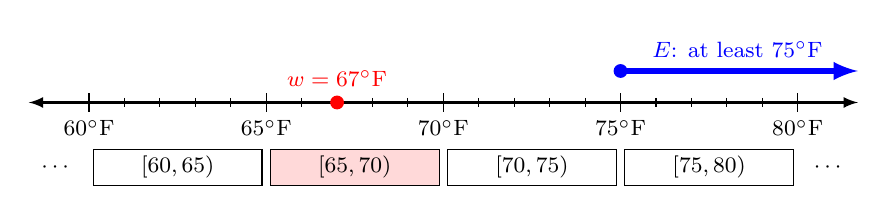
\begin{tikzpicture}[x=0.45cm, y=1cm, font=\footnotesize]
  \path (58.3,0.95) rectangle (81.7,-1.1); % fixed size so overlays don't shift the picture
  % number line
  \draw[latex-latex, thick] (58.3,0) -- (81.7,0);
  \foreach \t in {61,...,79} \draw (\t,0.06) -- (\t,-0.06);
  \foreach \t in {60,65,...,80} {
    \draw (\t,0.12) -- (\t,-0.12);
    \node[below] at (\t,-0.1) {$\t^\circ$F};
  }
  % state
  \fill<2->[red] (67,0) circle (2.5pt);
  \node<2->[above, red] at (67,0.08) {$w=67^\circ$F};
  % event
  \draw<3->[blue, line width=2pt, -latex] (75,0.4) -- (81.7,0.4);
  \fill<3->[blue] (75,0.4) circle (2.5pt);
  \node<3->[above, blue] at (78.3,0.45) {$E$: at least $75^\circ$F};
  % partition
  \fill<4->[red!15] (65.12,-0.6) rectangle (69.88,-1.05);
  \foreach \a [evaluate=\a as \b using int(\a+5)] in {60,65,70,75} {
    \draw<4-> (\a+0.12,-0.6) rectangle (\a+4.88,-1.05);
    \node<4-> at (\a+2.5,-0.825) {$[\a,\b)$};
  }
  \node<4-> at (59.1,-0.825) {$\cdots$};
  \node<4-> at (80.9,-0.825) {$\cdots$};
\end{tikzpicture}
\end{center}
\textbf{State (of the world)} $w$: a complete description of everything relevant
\begin{itemize}
    \item<1-> $W=$ set of all states \quad Ex: all temperatures
    \item<2-> \textbf{True state}: the one that actually happened \quad Ex: $67^\circ$F
    \item<3-> \textbf{Event} $E\subseteq W$: a set of states \quad Ex: ``at least $75^\circ$F''
\end{itemize}
\bsk
\onslide<4->{
\textbf{Information set} $I_i(w)$: the states Player $i$ thinks are possible when the truth is $w$
\begin{itemize}
    \item The info sets split up $W$: a \textbf{partition}
    \item Ex: P1's thermometer only shows $5^\circ$ bands: $I_1(67^\circ)=[65,70)$
    \item Coarse partition: knows little. Fine partition: knows a lot
\end{itemize}
}
\vfill
{\footnotesize Same word as ``information set'' in game trees. Same idea: ``where could I be?''}
\vspace{-0.2in}
\end{frame}

\begin{frame}{Example: Quiz Tomorrow?}
Alex was in class. Blair skipped. Alex texts Blair if there's a quiz\\ Texts sometimes get lost
\bsk
\begin{columns}[c]
\begin{column}{0.48\textwidth}
\begin{itemize}
    \item $\alpha$: quiz, Blair got the text
    \item $\beta$: quiz, text got lost
    \item $\gamma$: no quiz (no text)
\end{itemize}
\bsk
True state: $\alpha$
\end{column}
\begin{column}{0.5\textwidth}
\centering
\quizparts[0.68in]{}
\end{column}
\end{columns}
\bsk
\onslide<2->{Alex can't tell $\alpha$ from $\beta$. Why? \ans[3]{2.4in}{Can't see whether the text arrived}\\[4pt]
Blair can't tell $\beta$ from $\gamma$. Why? \ans[3]{2.4in}{No text either way}}
\vspace{-0.3in}
\end{frame}

\begin{frame}{Knowledge}
\textbf{In words:} $i$ knows $E$ at $w$ if \textbf{every} state $i$ thinks is possible is in $E$
$$w\in K_iE \iff \underbrace{I_i(w)}_{\text{what $i$ thinks is possible}}\ \subseteq\ \underbrace{E\vphantom{I_i(w)}}_{\text{the event}}$$
\begin{columns}[c]
\begin{column}{0.5\textwidth}
\centering
\quizparts[0.68in]{}
\end{column}
\begin{column}{0.48\textwidth}
$Q=$ ``quiz'' $=\{\alpha,\beta\}$
\bsk
$K_A Q=$ \ans{0.8in}{$\{\alpha,\beta\}$}\\[6pt]
$K_B Q=$ \ans{0.8in}{$\{\alpha\}$}
\bsk
At $\alpha$, who knows about the quiz? \only<2->{\alert{Both!}}
\end{column}
\end{columns}
\vspace{-0.3in}
\end{frame}

\begin{frame}{Knowing What Others Know}
``Blair knows $Q$'' is itself an event: $K_BQ=\{\alpha\}$
\bsk
\begin{columns}[c]
\begin{column}{0.5\textwidth}
\centering
\quizparts[0.68in]{}
\end{column}
\begin{column}{0.48\textwidth}
Does Alex know Blair knows?\\
$K_A K_B Q=$ \ans{0.8in}{$\emptyset$}
\bsk
Does Blair know Alex knows?\\
$K_B K_A Q=$ \ans{0.8in}{$\{\alpha\}$}
\end{column}
\end{columns}
\bsk
\onslide<3->{So at $\alpha$: both know there's a quiz. Blair knows Alex knows\\
But Alex \textbf{doesn't} know Blair knows!}
\vspace{-0.3in}
\end{frame}

\begin{frame}{Common Knowledge}
$E$ is \textbf{common knowledge} if: everyone knows $E$, everyone knows everyone knows $E$, everyone knows everyone knows everyone knows $E$, ... \textbf{forever}
\bsk
Infinitely many things to check?? No:
\bsk
\textbf{Reachable:} $w'$ is reachable from $w$ if you can get there in steps, where each step stays inside \textbf{someone's} information set
\bsk
\begin{block}{Fact (Bonanno \S8.3)}
$E$ is common knowledge at $w$ $\iff$ every state reachable from $w$ is in $E$
\end{block}
\bsk
Notation: $CK\,E$ $=$ states where $E$ is common knowledge
\vspace{-0.3in}
\end{frame}

\begin{frame}{Is the Quiz Common Knowledge?}
\centering
\only<1>{\quizparts{}}%
\only<2>{\quizparts{\draw[->, very thick, red!70] (0.08, 0.32) to[bend left=30] node[above, font=\small] {Alex} (0.92, 0.32);}}%
\only<3->{\quizparts{\draw[->, very thick, red!70] (0.08, 0.32) to[bend left=30] node[above, font=\small] {Alex} (0.92, 0.32);
  \draw[->, very thick, red!70] (1.08, -1.32) to[bend right=30] node[below, font=\small] {Blair} (1.92, -1.32);}}
\bsk
\raggedright
Starting at $\alpha$, which states are reachable? \ans[3]{1.2in}{$\alpha,\ \beta,\ \gamma$}
\bsk
\onslide<3->{$\gamma\notin Q$ $\Rightarrow$ the quiz is \textbf{not} common knowledge. Anywhere!}
\bsk
\onslide<4->{\textbf{Fact:} anything true at \textbf{every} state is common knowledge\\
\textbf{Ex:} ``Alex knows whether there's a quiz'' \ \textbf{Ex:} the game's rules (Ch.~14!)}
\vspace{-0.3in}
\end{frame}

\begin{frame}{Common Knowledge Is Rare, and Powerful}
Things that work because they create common knowledge:
\begin{itemize}
    \item \textbf{Public announcements:} ``Not all hats are white'' (Bonanno \S8.2)
    \item \textbf{Bank runs:} everyone sees the line around the block
    \item \textbf{Super Bowl ads:} you know everyone else saw it too
    \item \textbf{Read receipts:} ``Delivered'' vs.\ ``Read''
    \item \textbf{Protests:} I'll go if I know others will go...
\end{itemize}
\bsk
Private messages give knowledge. Public events give \textbf{common} knowledge
\vfill
{\footnotesize Not in the book. Chwe, \textit{Rational Ritual} (2001).}
\vspace{-0.2in}
\end{frame}

\begin{frame}{Adding Beliefs}
Each player puts \textbf{probabilities} on the states in each of their info sets
\bsk
\centering
\quizparts{\foreach \x/\y/\b in {0/0/{\tfrac{9}{10}}, 1/0/{\tfrac{1}{10}}, 2/0/1, 0/-1/1, 1/-1/?, 2/-1/?}
  {\node[anchor=east, font=\footnotesize, inner sep=1pt] at (\x-0.05, \y) {$\b$};}}
\bsk
\raggedright
\begin{columns}[T]
\begin{column}{0.45\textwidth}
Alex: texts arrive 90\% of the time
\end{column}
\begin{column}{0.53\textwidth}
Blair, with no text: Pr(quiz)?
\begin{itemize}
    \item Need to know: Pr(quiz) at all
    \item Say Pr(quiz) $=\tfrac12$
\end{itemize}
\end{column}
\end{columns}
\vfill
{\footnotesize Interactive knowledge-belief structure (Bonanno Def.~9.5.1): partitions plus beliefs.}
\vspace{-0.2in}
\end{frame}

\begin{frame}{Bayes' Rule}
\textbf{In words:} chance of $A$ once you learn $B$ $=$ share of $B$'s probability where $A$ is true
$$P(A\mid B)=\frac{\overbrace{P(A\cap B)}^{\text{$A$ and $B$}}}{\underbrace{P(B)}_{\text{all of $B$}}}$$
\bsk
Prior: $P(\alpha)=$ \ans{0.4in}{$.45$} \quad $P(\beta)=$ \ans{0.4in}{$.05$} \quad $P(\gamma)=$ \ans{0.4in}{$.50$}
\bsk
Blair gets no text, so learns $\{\beta,\gamma\}$:
$$P(\text{quiz}\mid\text{no text})=P(\beta\mid\{\beta,\gamma\})=\ans{1.4in}{$\dfrac{.05}{.05+.50}=\dfrac{1}{11}$}$$
\vspace{-0.3in}
\end{frame}

\begin{frame}{Back to Monty Hall}
You pick door 1. A state: (where the car is, which door Monty opens)
\bsk
\centering
\renewcommand{\arraystretch}{1.5}
\begin{tabular}{|c|c|c|}
\hline
State & Prior prob. & Monty opens \\
\hline
(Car 1, opens 2) & \ans{0.6in}{$\tfrac16$} & 2 \\
(Car 1, opens 3) & \ans{0.6in}{$\tfrac16$} & 3 \\
(Car 2, opens 3) & \ans{0.6in}{$\tfrac13$} & 3 \\
(Car 3, opens 2) & \ans{0.6in}{$\tfrac13$} & 2 \\
\hline
\end{tabular}
\bsk
\raggedright
Monty opens 3. Your info set: \ans{2.6in}{\{(Car 1, opens 3), (Car 2, opens 3)\}}\\[4pt]
$P(\text{car 1}\mid\text{opens 3})=$ \ans{1.1in}{$\dfrac{1/6}{1/6+1/3}=\dfrac13$} \quad Switch? \ans{0.5in}{Yes!}
\bsk
MobLab: \underline{\hspace{0.5in}}\% switched
\vspace{-0.3in}
\end{frame}

\begin{frame}{Common Prior}
\textbf{Common prior}: one probability $p$ on $W$ that gives \textbf{everyone's} beliefs by Bayes' rule
\bsk
\textbf{Ex:} Alex at $\{\alpha,\beta\}$: $(\tfrac{9}{10},\tfrac{1}{10})$. \ Blair at $\{\beta,\gamma\}$: $(\tfrac{1}{11},\tfrac{10}{11})$. Find $p$:\\[0.22in]
\onslide<2->{\alert{$p(\alpha)=9\,p(\beta)$ and $p(\gamma)=10\,p(\beta)$ \ $\Rightarrow$ \ $p=\left(\tfrac{9}{20},\ \tfrac{1}{20},\ \tfrac{10}{20}\right)$}}\\[0.22in]

\onslide<3->{\textbf{Why we care:} in Chapter 14, the common prior tells ``Nature'' how often to pick each state}
\bsk
\onslide<4->{\textbf{Fact:} a common prior doesn't always exist}
\vfill
{\footnotesize Bonanno Def.~9.5.2. Existence of a common prior is also called \textbf{Harsanyi consistency}.}
\vspace{-0.2in}
\end{frame}

% ---- MobLab run: Herding (Information Cascade) ------------------------
% Macro and Finance topic. Default majority 60%. Groups of 5-6, random
% order. A few periods. Played at the end of deck 11 (moved here from
% deck 12), as an application of Bayes' rule. Debrief follows directly
% in "Back to Herding".
% ---------------------------------------------------------------------
\begin{frame}{MobLab: ``Herding (Information Cascade)''}
\begin{itemize}
    \item MobLab time!
    \item A jar is either mostly \textbf{Blue} or mostly \textbf{Red} (equally likely)
    \begin{itemize}
        \item Mostly $=$ 60\% of the balls
    \end{itemize}
    \item You privately draw one ball (it goes back in)
    \item One at a time, in random order, guess: Blue jar or Red jar?
    \begin{itemize}
        \item You see everyone's \textbf{guesses} before you. Not their balls
    \end{itemize}
    \item Paid for a correct guess
\end{itemize}
\vfill
\centering
Feel free to talk! And play it the way you'd actually play it.
\vspace{-0.2in}
\end{frame}

\begin{frame}{Back to Herding}
Suppose everyone guesses their own ball's color... until it stops making sense
\bsk
\textbf{Player 2} sees ``Blue'', draws blue:\\
$P(\text{Blue jar})=\dfrac{(.6)(.6)}{(.6)(.6)+(.4)(.4)}=$ \ans{0.9in}{$\dfrac{9}{13}\approx .69$}
\bsk
\textbf{Player 3} sees ``Blue, Blue'', draws \textbf{red}:\\
Two blue balls revealed, one red. $P(\text{Blue jar})=$ \ans{0.6in}{$.6$} \ Guess? \ans{0.5in}{Blue}
\bsk
\onslide<3->{\textbf{Cascade:} from now on, guesses reveal nothing. Everyone herds}\\
\onslide<4->{This is \textbf{Bayes' rule} at work: early guesses reveal balls, later guesses don't\\
Our groups: \underline{\hspace{0.4in}} cascades, \underline{\hspace{0.4in}} on the wrong color}
\vfill
{\footnotesize Anderson \& Holt (1997, \textit{AER}). Not in the book.}
\vspace{-0.2in}
\end{frame}

% ==============================================================
% WORKED EXAMPLE
% ==============================================================
% Answers are in the header comment.
% ---------------------------------------------------------------------

\begin{frame}[standout]
Let's Work One Out
\end{frame}

\begin{frame}{Kickoff Time}
\begin{columns}[c]
\begin{column}{0.48\textwidth}
\centering
\begin{tikzpicture}[x=0.65in, y=0.55in]
  \foreach \x/\s/\p in {0/a/.1, 1/b/.2, 2/c/.3, 3/d/.4} {\node at (\x, 0.75) {$\s$}; \node[font=\scriptsize, text=gray] at (\x, -1.75) {\p};}
  \node[anchor=east, text=player1] at (-0.35, 0) {Jordan:};
  \node[anchor=east, text=player2] at (-0.35, -1) {Casey:};
  \foreach \x in {0,1,2,3} {\fill (\x, 0) circle (2pt); \fill (\x, -1) circle (2pt);}
  \draw[player1, thick, rounded corners=7pt] (-0.25, -0.25) rectangle (1.25, 0.25);
  \draw[player1, thick, rounded corners=7pt] (1.75, -0.25) rectangle (3.25, 0.25);
  \draw[player2, thick, rounded corners=7pt] (-0.25, -1.25) rectangle (0.25, -0.75);
  \draw[player2, thick, rounded corners=7pt] (0.75, -1.25) rectangle (2.25, -0.75);
  \draw[player2, thick, rounded corners=7pt] (2.75, -1.25) rectangle (3.25, -0.75);
  \node[font=\scriptsize, text=gray, anchor=east] at (-0.35, -1.75) {prior:};
\end{tikzpicture}
\bsk
\raggedright
{\footnotesize Kickoff is at noon in $N=\{a,b,c\}$. True state $a$}
\end{column}
\begin{column}{0.5\textwidth}
\begin{enumerate}
    \item Find $K_J N$ and $K_C N$ \vspace{0.2in}
    \item At $a$, does Jordan know that Casey knows $N$? \vspace{0.2in}
    \item Is $N$ common knowledge at $a$? \vspace{0.2in}
    \item Use the prior to find each player's beliefs \vspace{0.25in}
    \item If Casey's beliefs at $\{b,c\}$ were $(\tfrac12,\tfrac12)$, is there still a common prior? \vspace{0.1in}
\end{enumerate}
\end{column}
\end{columns}
\vspace{-0.3in}
\end{frame}

\begin{frame}{What Have We Learned, Charlie Brown?}
\begin{itemize}
    \item \textbf{States} and \textbf{information partitions}: who can tell what apart
    \item $i$ knows $E$ at $w$ $\iff$ $I_i(w)\subseteq E$
    \item \textbf{Common knowledge}: every reachable state is in $E$
    \begin{itemize}
        \item True at every state $\Rightarrow$ common knowledge
    \end{itemize}
    \item \textbf{Beliefs}: probabilities on each information set
    \item \textbf{Bayes' rule}: $P(A\mid B)=P(A\cap B)/P(B)$
    \item \textbf{Common prior}: one $p$ that generates everyone's beliefs
    \item \textbf{Information cascade}: once guesses stop revealing signals, everyone herds
\end{itemize}
\vfill
\vspace{-0.4in}
\end{frame}

\begin{frame}{Reading \& Practice}
\begin{itemize}
    \item Bonanno, Chapter 8
    \begin{itemize}
        \item \S8.1--8.3: read. Skip \S8.4--8.5 (belief relations)
    \end{itemize}
    \item Bonanno, Chapter 9
    \begin{itemize}
        \item \S9.1--9.3 and \S9.4.1: read (probability, Bayes' rule)
        \item \S9.5: read (common prior). Skip \S9.4.2 and \S9.6--9.7
    \end{itemize}
    \item Exercises: \S8.6.1--8.6.3, \S9.8.3
    \item Solutions in \S8.7 and \S9.9. Try them first
\end{itemize}
\vfill
\end{frame}

\end{document}
